\section{Asservissement du moteur}

\subsection{Asservissement en courant du moteur}

\subsubsection{Modélisation sur Matlab/Simulink}

% image de l'asservissement en courant Simulink
\begin{figure}[H]
    \centering
    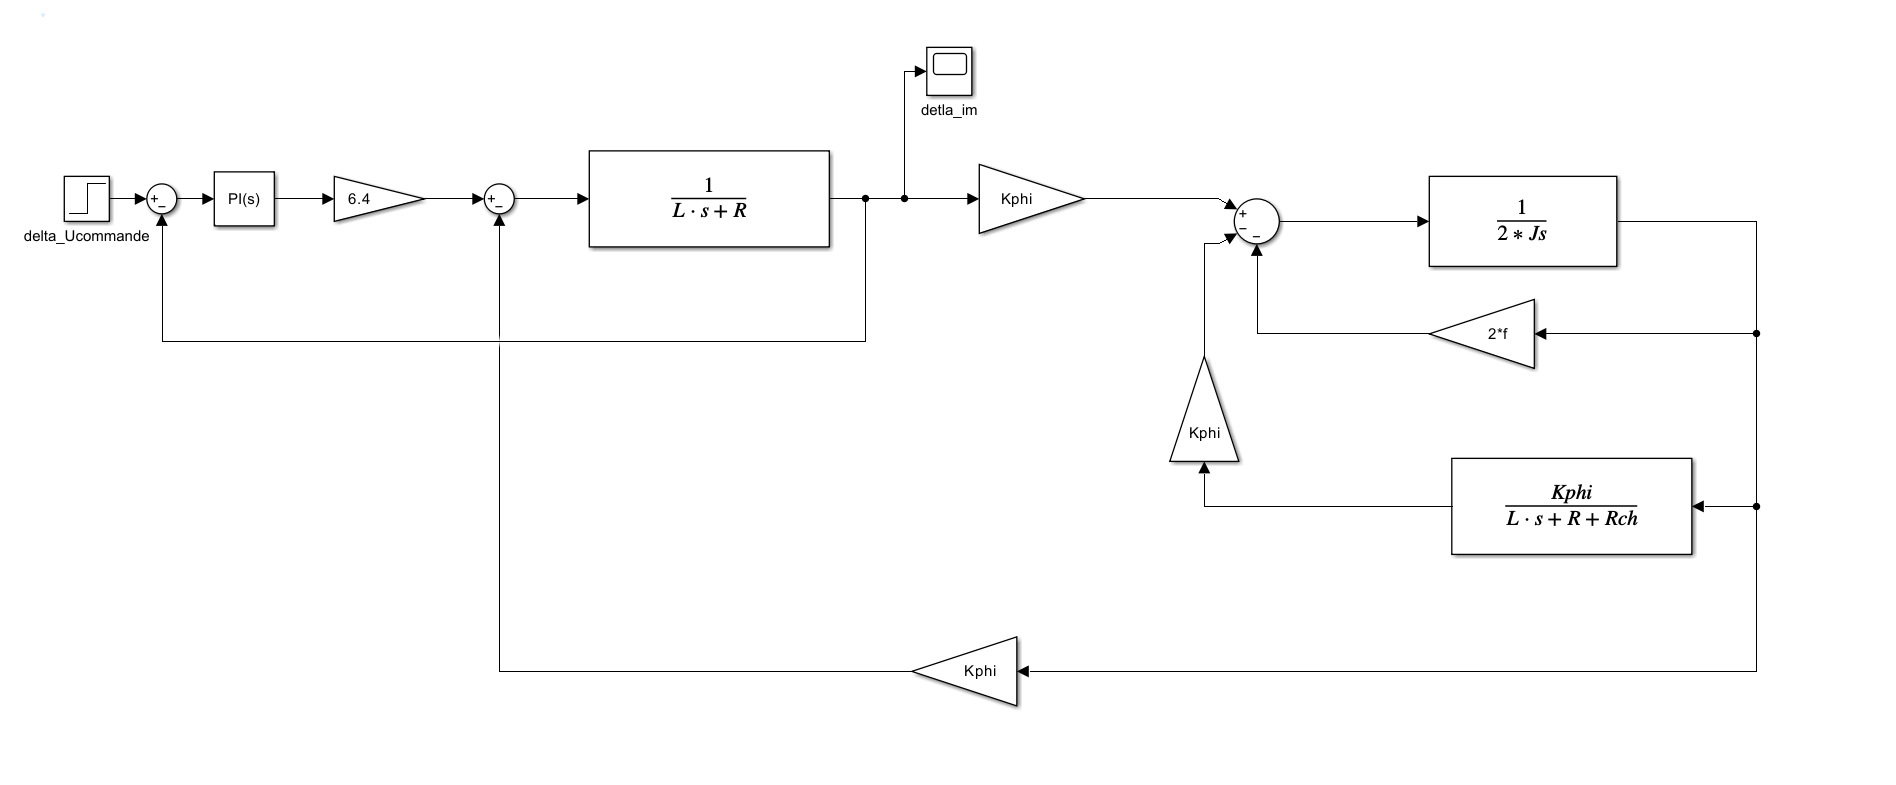
\includegraphics[width=1\textwidth]{images/boucle_de_courant/Simulink_boucle_de_courant.png}
    \caption{Schéma de l'asservissement en courant du moteur dans Simulink}
    \label{fig:asservissement_courant_simulink}
\end{figure}

% réponse indicielle de l'asservissement en courant Simulink
\begin{figure}[H]
    \centering
    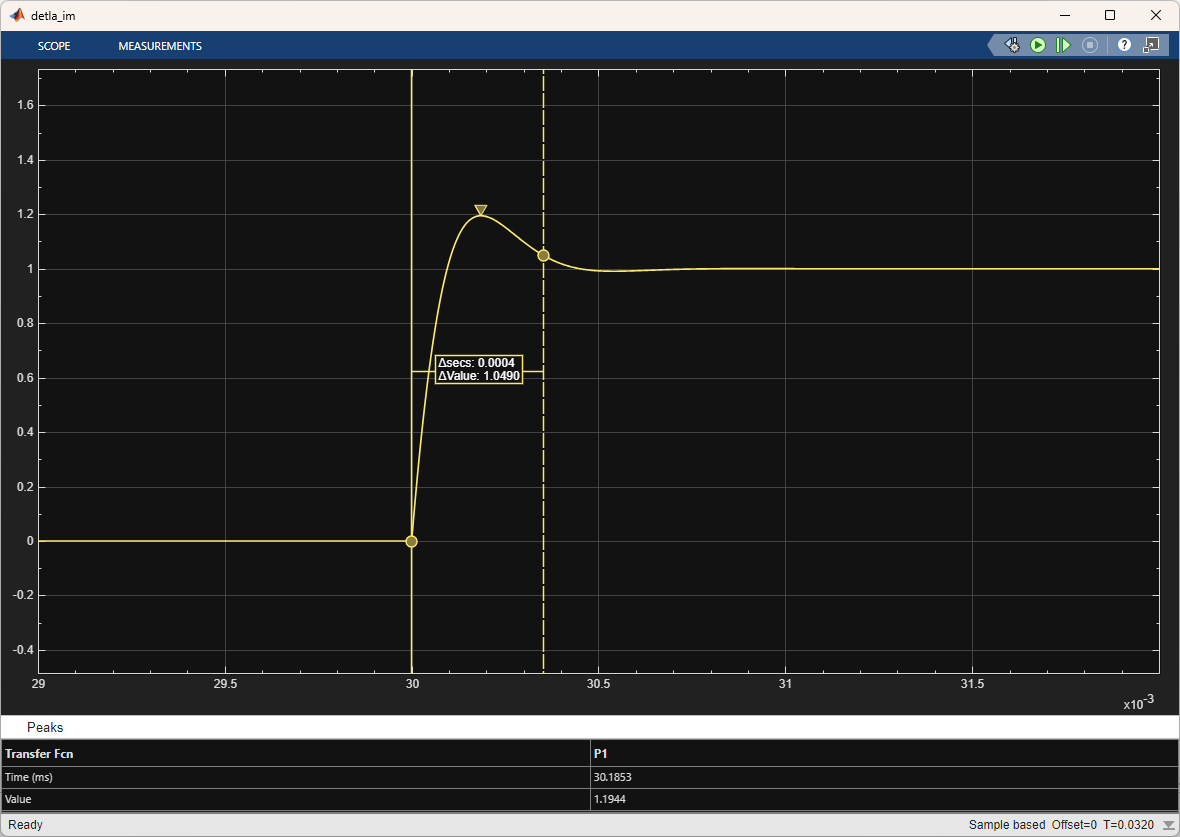
\includegraphics[width=1\textwidth]{images/boucle_de_courant/Simulink_reponse_indicielle_courant.png}
    \caption{Réponse indicielle de l'asservissement en courant du moteur dans Simulink}
    \label{fig:reponse_indicielle_courant_simulink}
\end{figure}

On constate que la réponse indicielle de l'asservissement en courant du moteur dans Simulink présente un dépassement d'environ 19\% et un temps de réponse de 0,35 ms. Ce qui respecte les spécifications du cahier des charges qui exige un dépassement maximal de 20\% et un temps de réponse maximal de 10 fois la prériode de la MLI soit 0,45 ms.

\subsubsection{Modélisation sur PSIM}

% image de l'asservissement en courant PSIM
\begin{figure}[H]
    \centering
    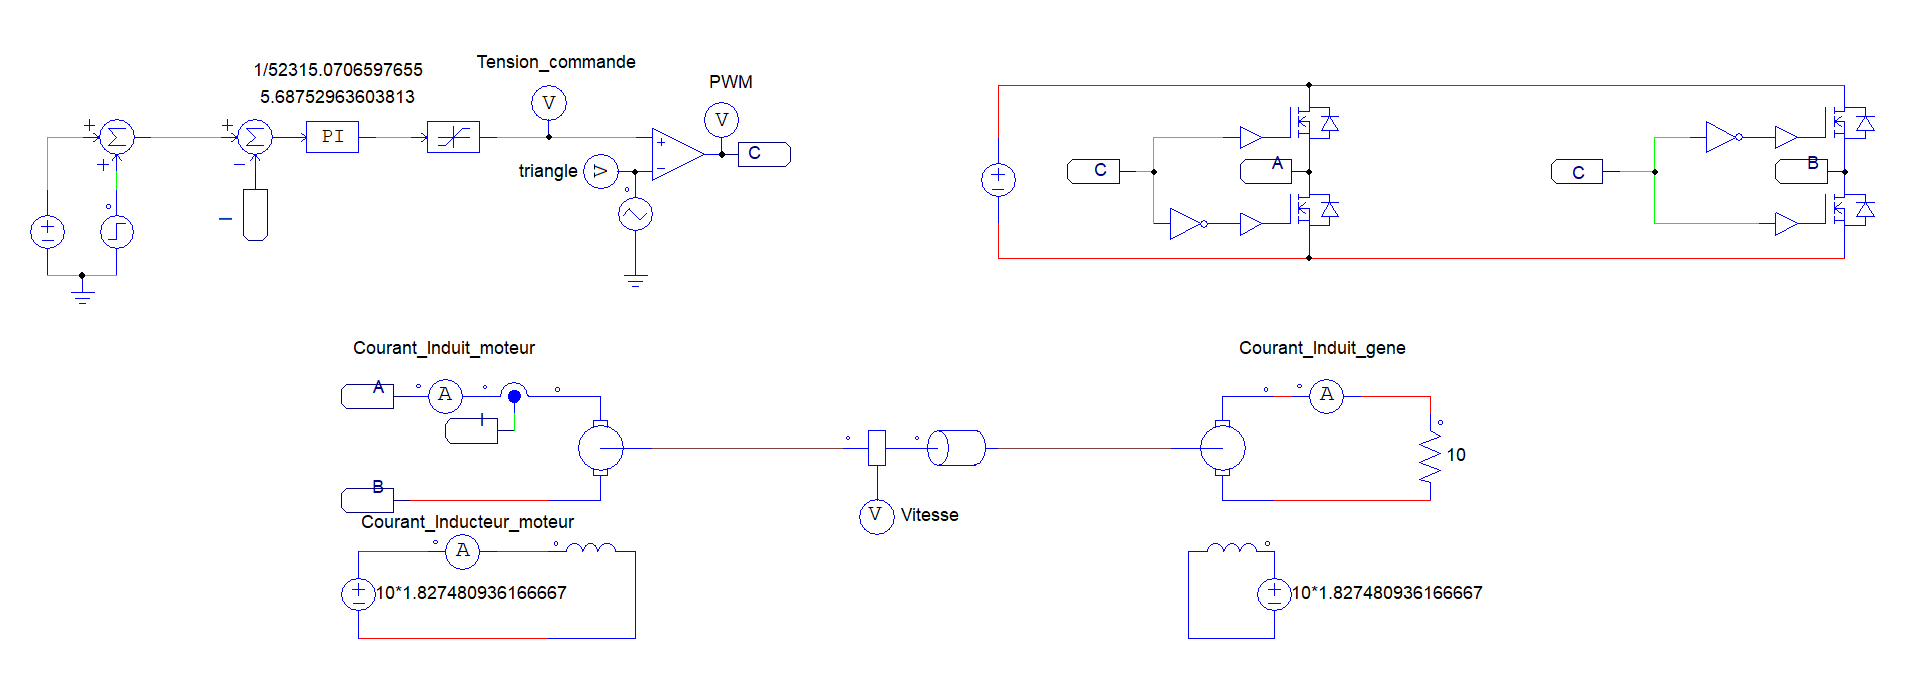
\includegraphics[width=1\textwidth]{images/boucle_de_courant/PSIM_boucle_de_courant.png}
    \caption{Schéma de l'asservissement en courant du moteur dans PSIM}
    \label{fig:asservissement_courant_psim}
\end{figure}
% réponse indicielle de l'asservissement en courant PSIM
\begin{figure}[H]
    \centering
    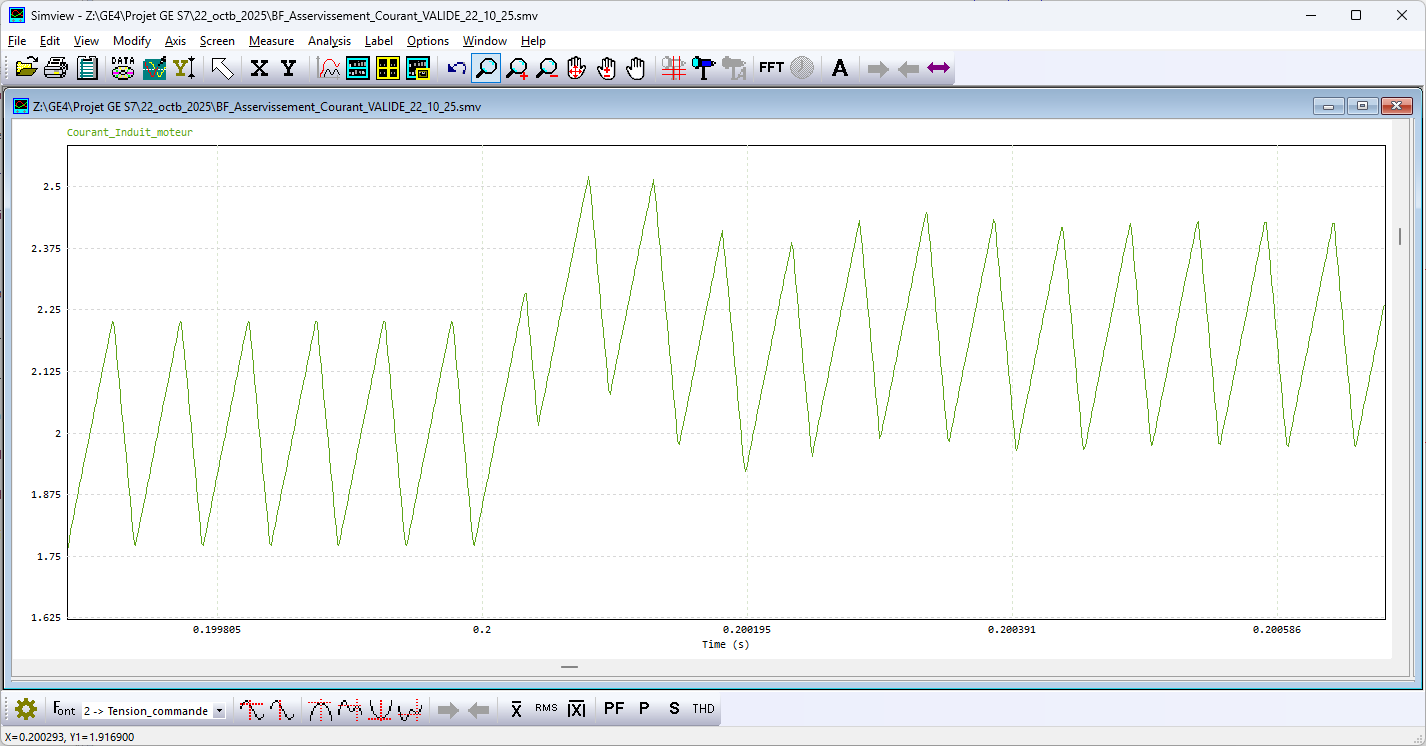
\includegraphics[width=1\textwidth]{images/boucle_de_courant/PSIM reponse indicielle courant BF.png}
    \caption{Réponse indicielle de l'asservissement en courant du moteur dans PSIM}
    \label{fig:reponse_indicielle_courant_psim}
\end{figure}

\subsubsection{Comparaison des résultats}

Dans cette section, nous allons comparer les résultats obtenus avec les deux outils de simulation, Simulink et PSIM.

% image de la comparaison des réponses
\begin{figure}[H]
    \centering
    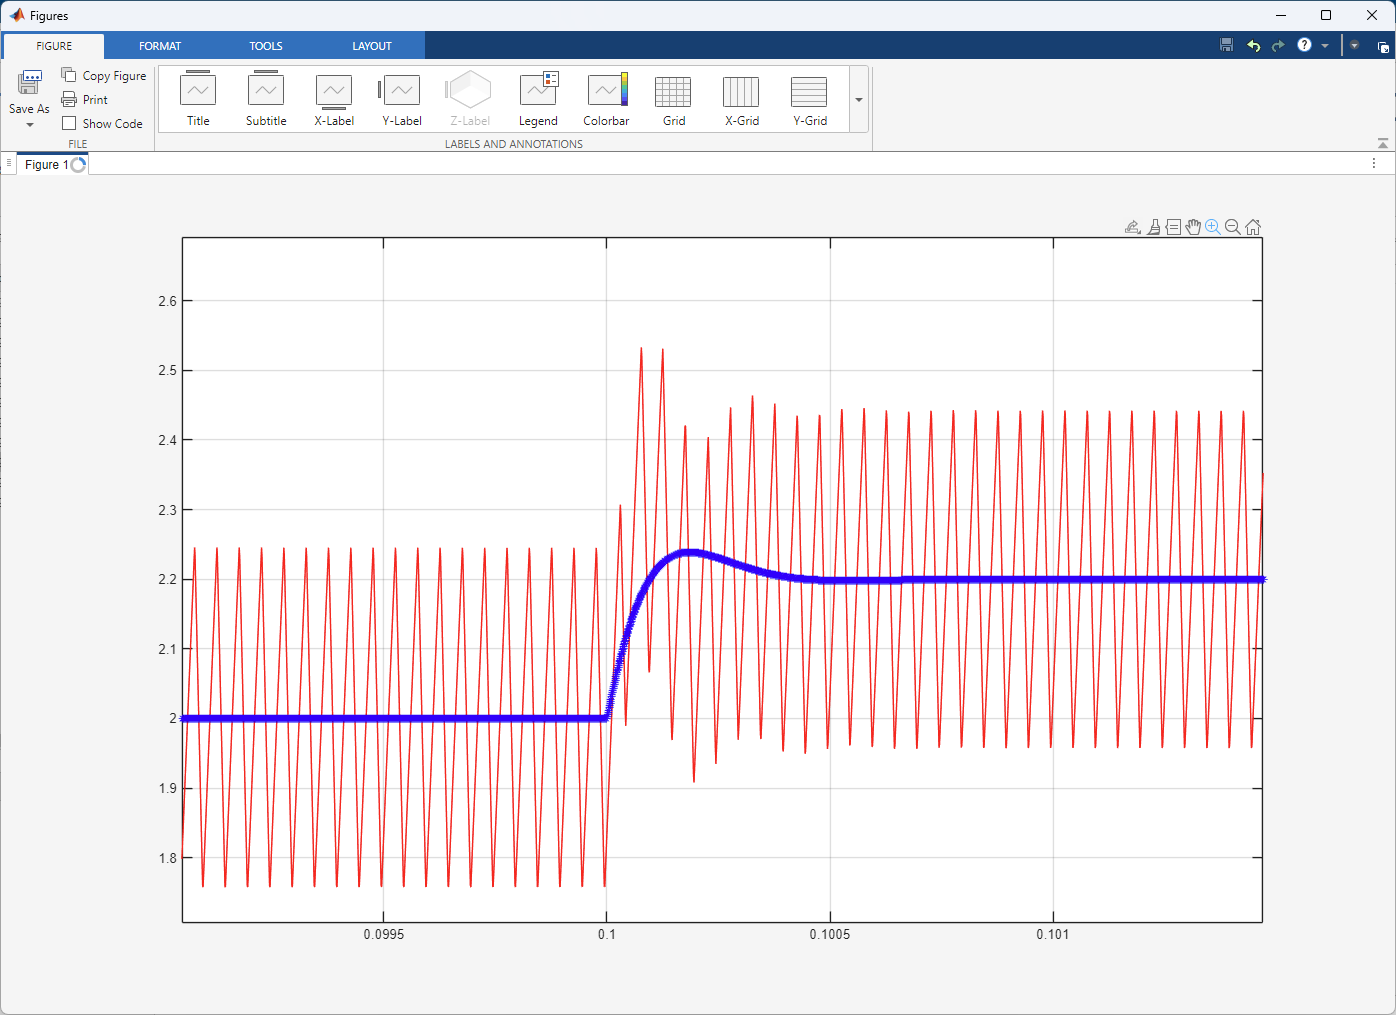
\includegraphics[width=1\textwidth]{images/boucle_de_courant/comparaison_reponse_indicielle_courant.png}
    \caption{Comparaison des réponses indicielle de l'asservissement en courant du moteur entre Simulink et PSIM}
    \label{fig:comparaison_reponse_indicielle_courant}
\end{figure}

\subsection{Asservissement en vitesse du moteur}

\subsubsection{Simulation sur Matlab/Simulink}
Nous commencons par la simulation de la vitesse du moteur en boucle ouverte sur Simulink. 

% réponse de l'asservissement en vitesse Simulink
\begin{figure}[H]
    \centering
    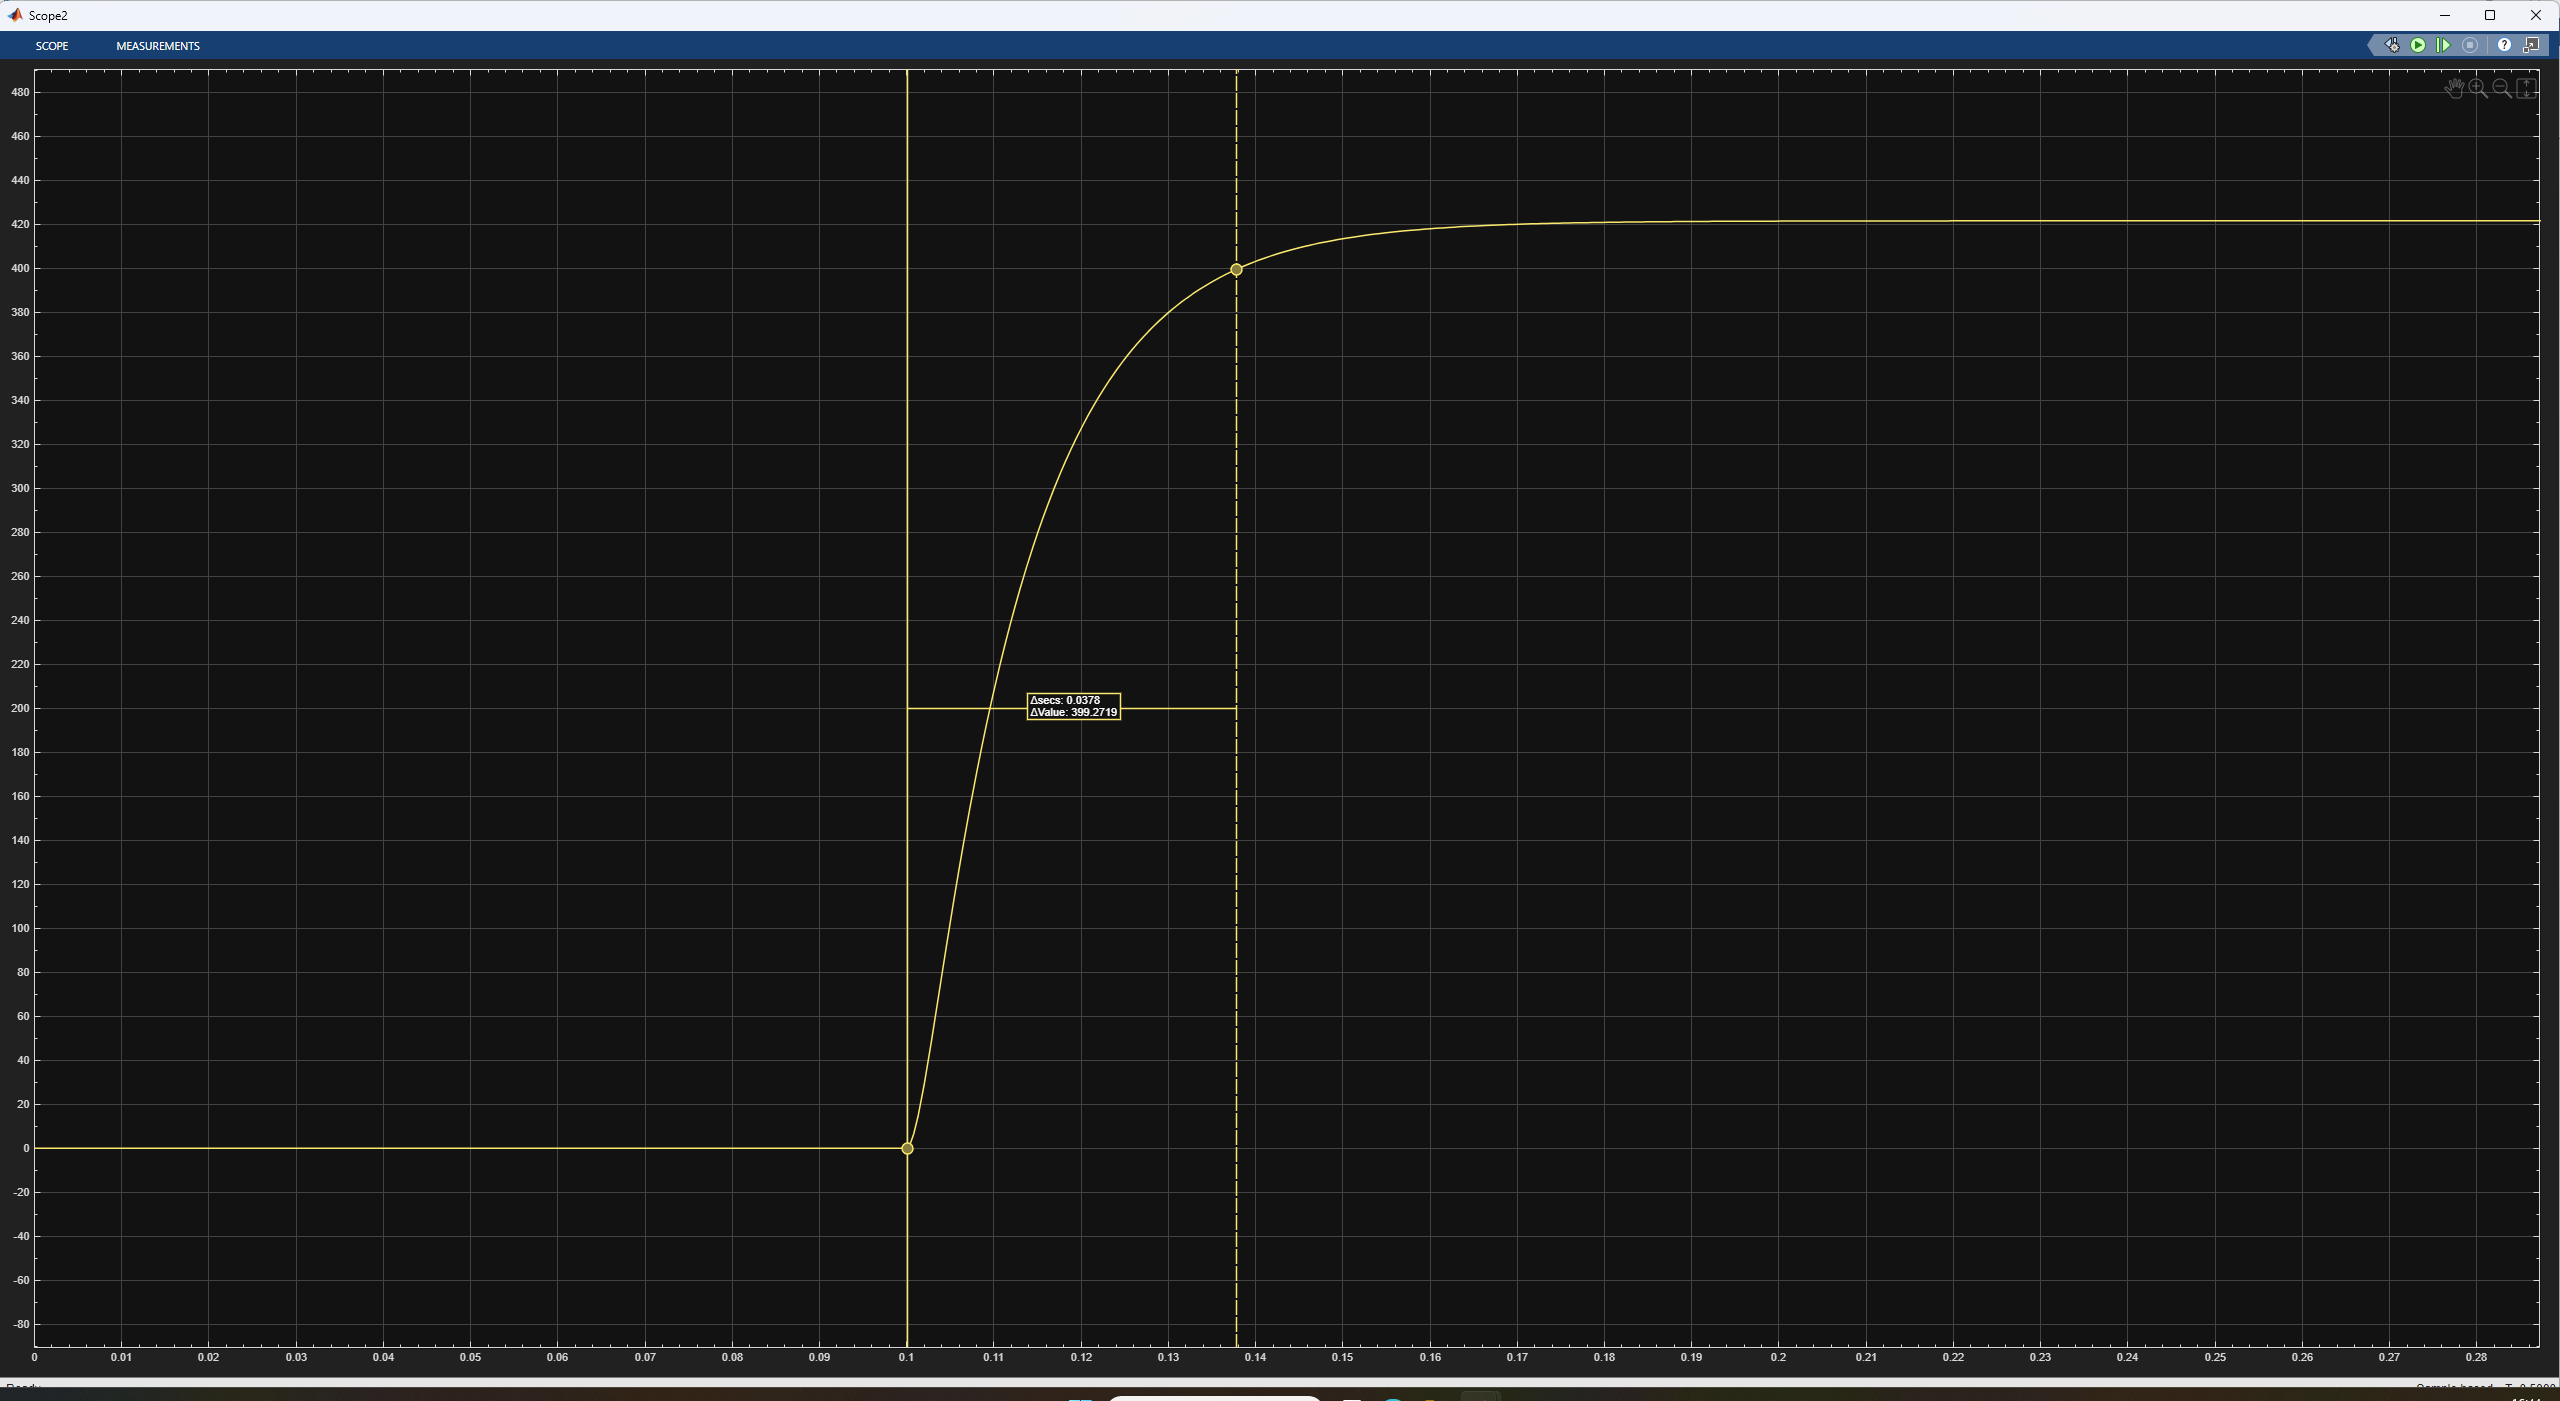
\includegraphics[width=1\textwidth]{images/asserv_de_vitesse_tachy/Vitesse_tr5_BO.png}
    \caption{Réponse de la vitesse du moteur en boucle ouverte dans Simulink}
    \label{fig:asservissement_vitesse_simulink}
\end{figure}
On releve un temps de réponse à 5\% en boucle ouverte pour la vitesse, sur Simulink : 37,8 ms

Nous cherchons ensuite à asservir la vitesse du moteur en boucle fermée avec un correcteur PI. Nous visons un temps de réponse à 5\% 3 fois plus rapide qu'en boucle ouverte soit 12,6 ms avec un dépassement maximal de 20\%.
\begin{figure}[H]
    \centering
    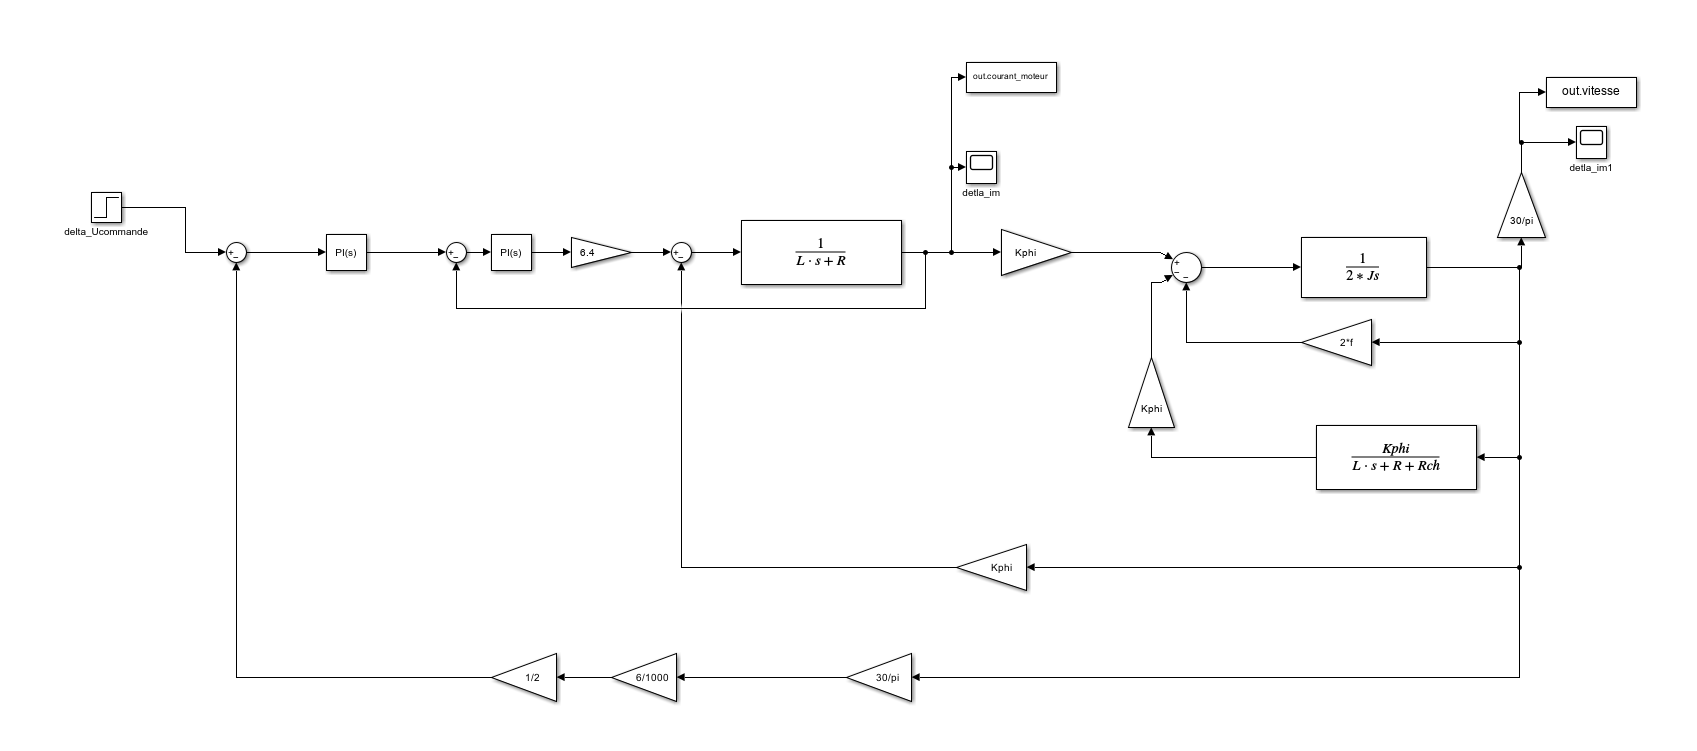
\includegraphics[width=1\textwidth]{images/asserv_de_vitesse_tachy/Simulink_boucle_de_courant_vitesse.png}
    \caption{Schéma de l'asservissement en vitesse du moteur dans Simulink}
    \label{fig:asservissement_vitesse_simulink_schema}
\end{figure}
A l'aide du PID Tuner de Simulink, nous obtenons les valeurs suivantes pour le correcteur PI :
\begin{itemize}
    \item $K_p = 37,3376029909659$
    \item $K_i = 14022,585396076$
\end{itemize}
% réponse de l'asservissement en vitesse Simulink
\begin{figure}[H]
    \centering
    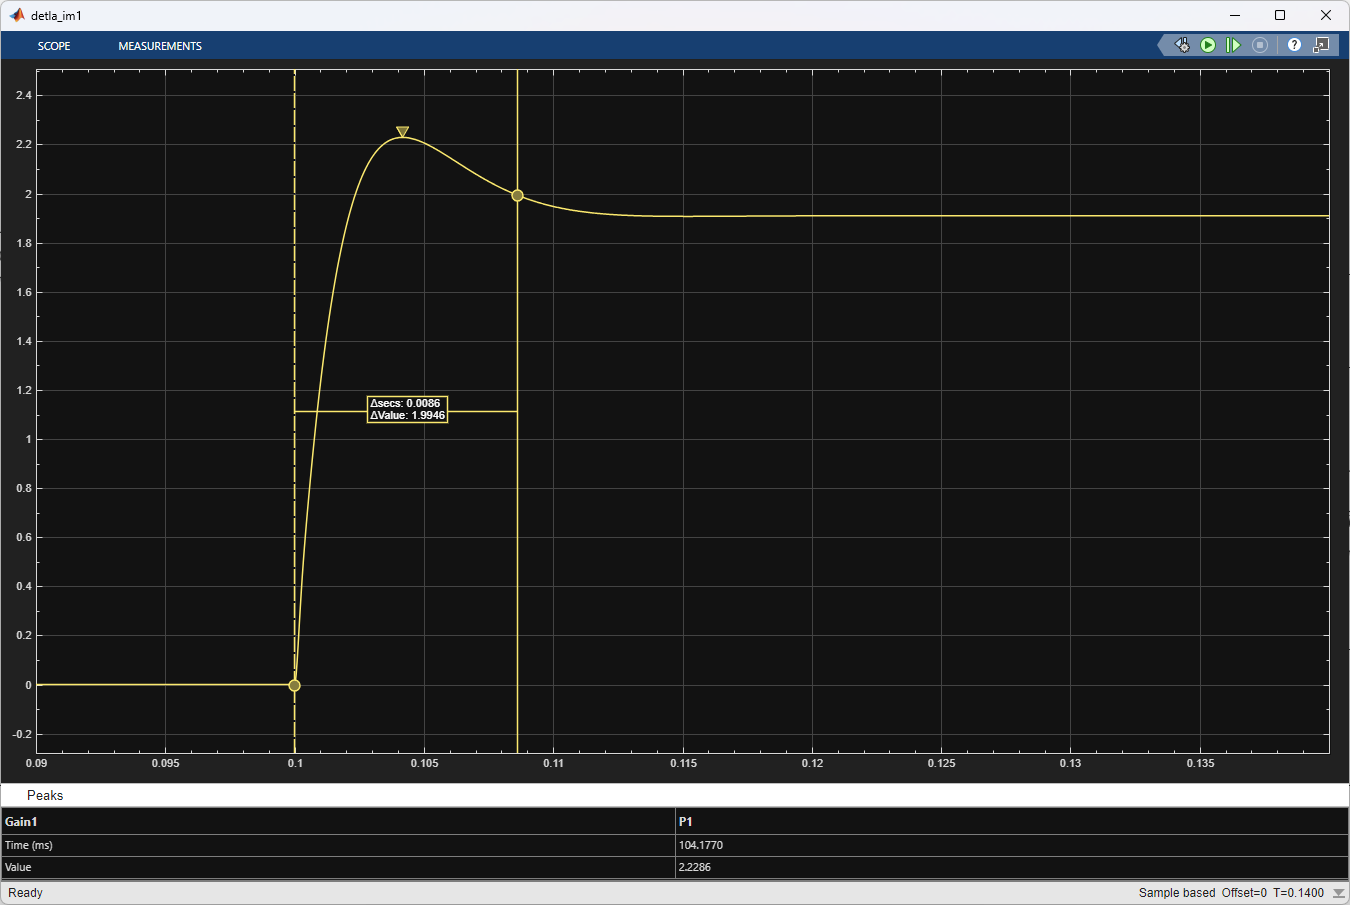
\includegraphics[width=1\textwidth]{images/asserv_de_vitesse_tachy/Vitesse_tr5_BF.png}
    \caption{Réponse de l'asservissement en vitesse du moteur dans Simulink}
    \label{fig:reponse_asservissement_vitesse_simulink}
\end{figure}
Nous relevons un temps de réponse à 5\% de 7,6 ms et un dépassement de 18,5\%, ce qui respecte les spécifications du cahier des charges.

\subsubsection{Simulation sur PSIM}

\subsubsection{Comparaison des résultats}

\subsection{Asservissement en vitesse avec le codeur incrémental}
Le cahier des charges impose la possibilité d'asservir la vitesse du moteur à l'aide d'un codeur incrémental.
\subsubsection{Principe de fonctionnement du codeur incrémental}

Le fonctionnement du codeur incrémental repose sur un disque rotatif équipé de fentes. Celui-ci est interposé entre une diode électroluminescente et un capteur photodiode. Lorsque le disque tourne, les fentes permettent à la lumière de passer à travers, générant ainsi des impulsions électriques dans le capteur. Le nombre d'impulsions générées par tour dépend de la résolution du codeur.
\\\\
Le codeur incrémentale fournit est composé de deux piste de fentes decalé d'un quart de période, ce qui permet de déterminer le sens de rotation du moteur en analysant la séquence des impulsions générées par les deux capteurs. 
\\\\
Pour mesurer la vitesse de rotation du moteur, il suffit de compter le nombre d'impulsions générées par le codeur sur une période de temps donnée. La vitesse angulaire peut être calculée en utilisant la formule suivante :
\begin{equation}
    \omega = \frac{N \cdot 2\pi}{P \cdot T}
\end{equation}
où :
\begin{itemize}
    \item $\omega$ est la vitesse angulaire en radians par seconde (rad/s)
    \item $N$ est le nombre d'impulsions comptées
    \item $P$ est le nombre d'impulsions par tour du codeur
    \item $T$ est la période de temps pendant laquelle les impulsions sont comptées en secondes (s)
    \item $2\pi$ est une constante pour convertir les tours en radians
\end{itemize}

Pour connaitre le sens de rotation, on analyse la séquence des impulsions des deux pistes. Si la piste A précède la piste B, le moteur tourne dans un sens. Si la piste B précède la piste A, le moteur tourne dans le sens inverse.
